%chapter 3:
%1. The power of model based approach--> one wall sample and one pincecess can solve the whole maze problem
   %1.1. show the effectiveness
   %1.2. scaling up--> a noval biased model-based approach (show that it is the only way)
   %1.3. the necessity of biased approach
   %1.4. the choice between planning variable and not
   %1.5. wrong decision variable causes disater (decision)

%chapter 4:
%1. the three optimality ()
%2. Combined with hierarchical optimal RL
%3. why we need leaf cover
%4. the convergence for online approach
%5. the offiline one
%6. Respect the hierarchy

%chapter 5:
%1. why my modification, the hierarchy will not be destoryed (the overhead of adding additional action is small)
%2. The hierarchy is destoryed with HORDQ
%3. The pseudo reward can enforce the hierarchical policy

%MAXQ (include the algorithm), hierarchical optimal vs recursive optimal, HORDQ, Relational,  Model-based RL (cite Peter Stone's Model based approach and a brief intro of it, include the algorithm)
%the problem of HO
%Optimal planning, model the differences

%TODO: say that it is possible to use any hierarchically optimal RL algorithm to obtain the same result here with diffrent 
%proof, , but the benefit of HORDQ is ...
\chapter{Learning}

%An overview here
In this chapter, we show how to exploit the property of hierarchical optimal reinforcement learning
to help model-based methods learn the optimal policy by combining them with model-free methods.
The main idea is to exploit the fact that a hierarchically optimal reinforcement learning method allows 
a subtask to know the "consequence" of its own action, thus it will pursue a subgoal
only when it leads to the optimal policy. It allows the subtask to act optimally 
regardless of which subgoal is set by its parent subtask.

%The difference of recursively optimal policy and hierarchically optimal policy is explained
%in section \ref{se:ROHO}. 


However, a hierarchically optimal method alone cannot guarantee that the optimal 
policy can be always learned. To ensure that the optimal policy can be learned, 
we need to "patch" the hierarchy to allow some subtasks to be able to solve
the whole MDP on their own. The result is presented in section \ref{se:OptimalPlanning}.

It is worth noting that
what we are seeking here is optimality, not
recursive optimality nor hierarchical optimality.
Since we allow some of subtasks to learn a suboptimal policy,
the recursive optimality cannot be achieved.
The hierarchical optimality cannot be achieved as well before the hierarchy is patched.
In Theorem \ref{thm:opt}, we show that the hierarchically optimal policy
is equal to optimal policy with a patched hierarchy.
In other words, seeking the optimality or hierarchical optimality are the same
with a patched hierarchy. 
%TODO: what we seek is optimality not RO or HO

In this work, we follow a hierarchical formulation that is similar to the MAXQ framework \cite{MaxQJ}.
An MDP $M$ is decomposed into a finite
set of subtasks $M' = \{M_0, M_1, \dots, M_n\}$, where $M_0$ is the root subtask. 
Each subtask is defined by 3 tuples $<U_i, A_i, R_i>$, where 
$U_i$ is a termination predicate that partitions the state space into active states $S_i$ and terminal states $T_i$,
$A_i$ is a set of actions for subtask $M_i$,
and $R_i$ is the reward function for subtask $M_i$.
There are two types of actions: primitive and composite.
A primitive action corresponds to one of the actions in MDP $M$, which takes one step to finish. 
A composite action corresponds to a subtask in the hierarchy, which will not finish before
the subtask arrive one of its terminal states.

Different from MAXQ, 
the reward function $R_i$ is separated into internal reward function and external reward function.
The internal reward function is equivalent to the reward function of MAXQ. It defines the pseudo-reward that
encourages the agent to pursue the subgoal of each subtask.
The internal reward function is defined for terminal states, and zero elsewhere.
The external reward function is identical to the reward function of MDP $M$.
It encourages the agent to pursue the goal defined by the original MDP $M$.
The analysis in section \ref{se:OptimalPlanning} assumes the pseudo-reward is zero everywhere.
The issues with the pseudo-reward are discussed in section \ref{se:pseudo}.

\section{Optimal planning with task hierarchy}
\label{se:OptimalPlanning}

\begin{figure}[t]
\begin{center}
    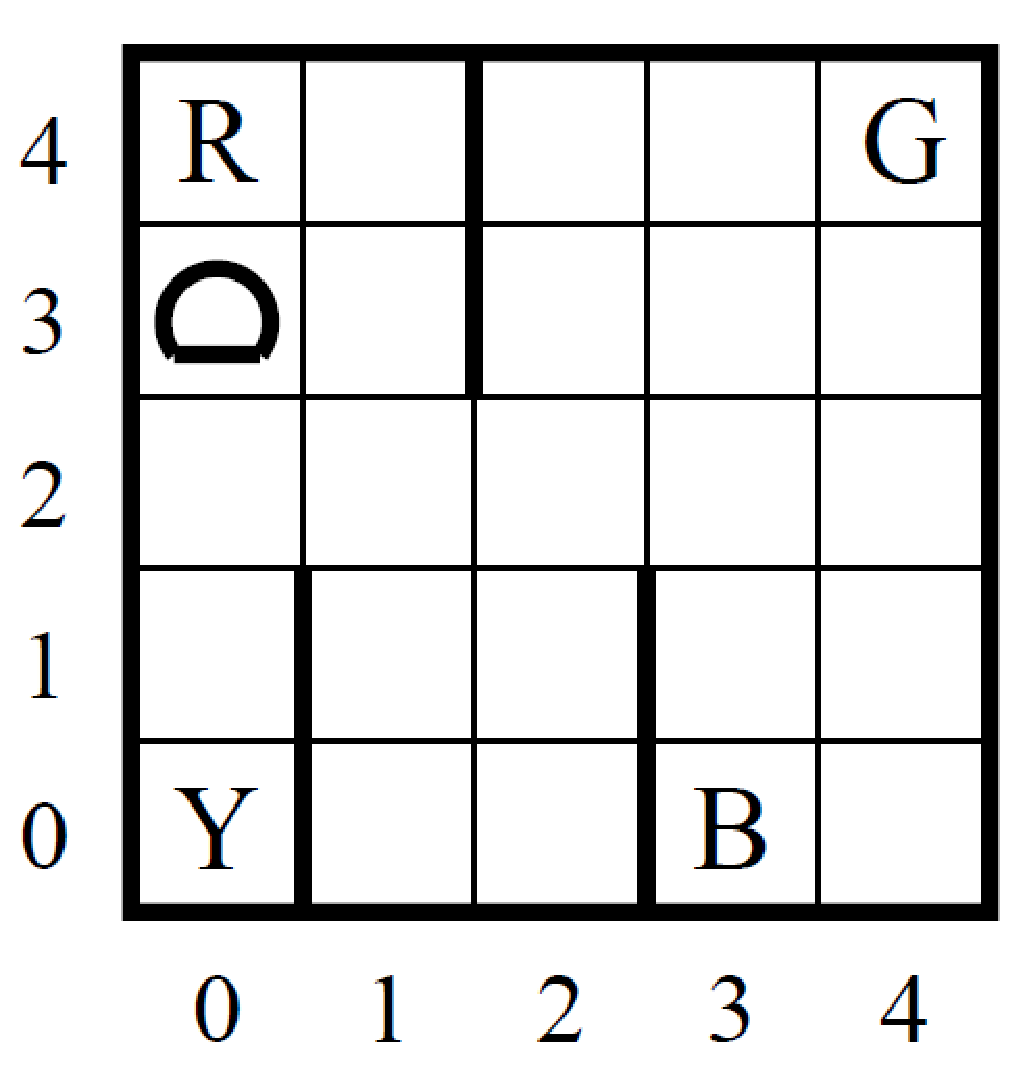
\includegraphics[width=4.5in] {./figures/taxi.eps}
\end{center}
\caption{The Taxi Domain.}
\label{fig:taxi_domain}
\end{figure}

\begin{figure}[t]
\begin{center}
    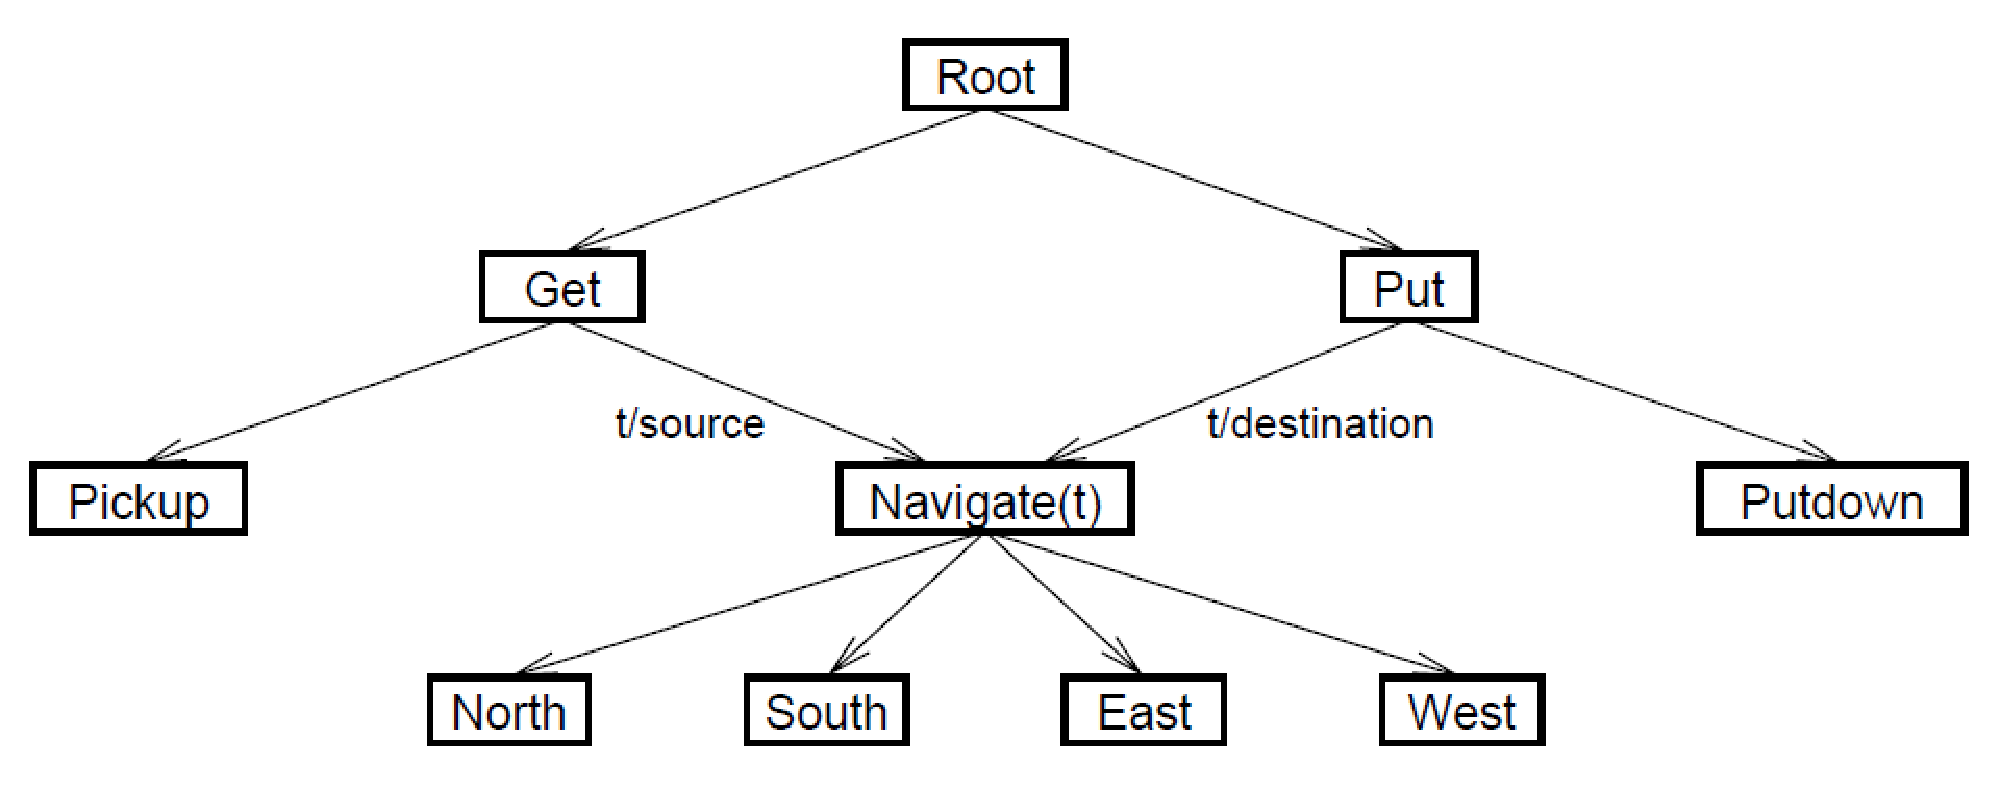
\includegraphics[width=4.5in] {./figures/TaxiHierarchy.eps}
\end{center}
\caption{The task hierarchy of Taxi domain.}
\label{fig:taxi}
\end{figure}

We illustrate our idea with the task hierarchy of Taxi domain \cite{MaxQJ} (Fig. \ref{fig:taxi, fig:taxi_domai}).
The taxi problem is an episodic task. For each episode, the taxi starts
at a random location. To finish the task, the taxi needs to go to the passenger's location, pick up the passenger,
go to the destination, and put down the passenger. The task can be further decomposed two subtasks: $Get$ and $Put$. 
The goal of subtask $Get$ is to move the taxi to the passenger's location and pick up the passenger. The goal of 
subtask $Put$ is to put down the passenger at the destination.

Assume the policy of subtask $Root$ is suboptimal and always invokes $Get$ even when 
the passenger is already in the taxi. Optimality can be guaranteed if subtask $Get$
learns to deliver the passenger to his destination.
Or suppose the policy of $Root$ always chooses $Put$.
If subtask $Put$ learns to pickup the passenger when he is not in the taxi, 
we will have the optimal policy because it does not matter which decision is made 
by $Root$, the passenger can always be picked up and delivered to the destination.

The above example provides two observations.
First, in order to guarantee optimality, subtasks $Get$ and $Put$ need 
to act optimally in regards to the goal of whole problem, not 
the subgoal of each subtask. It implies that we need to seek hierarchical optimality
rather than recursive optimality.

Second, optimality cannot be guaranteed without modification of the hierarchy. In the original hierarchy, 
subtask $Get$ has no access to action $Putdown$. Even though subtask $Get$ delivers the passenger to the destination,
it cannot put him down. We need to modify the hierarchy to let subtask $Get$ be
able to solve the problem on its own. A way to achieve that is to let subtask $Get$ have access
to action $Putdown$. 

%We can only guarantee optimality by adopting HORDQ for certain positions
%in the hierarchy. The "positions" are defined by the following definition:

We define which subtasks shall act optimally with the following definition:
\begin{definition}
    $C(H) = \{M_{j_1}, M_{j_2}, \dots, M_{j_k}\}$ is a leaf cover of hierarchy $H$ 
    if there is no subtask $M_i \notin C(H)$ which has access to a primitive action.
    Furthermore, $TC(H)$ is a total leaf cover if it is a leaf cover and all primitive
    actions are directly or indirectly (through child subtasks) accessible for every 
    subtask $M_i \in TC(H)$.
\end{definition}

%A leaf cover contains the subtasks which are able to solve the problem on their own.
We can always find a leaf cover for a hierarchy by including all subtasks which have access
to primitive actions. The total leaf cover can be constructed from the leaf cover by
adding the missing primitive actions.
Consider the task hierarchy in the Taxi domain in Figure \ref{fig:taxi},
if we add action $Pickup$ and $Putdown$ to subtask $Navigate$, 
we get a total leaf cover which consists of subtasks $Get$, $Put$, and $Navigate$.
%Another way is to let Navigate, Get and Put subtasks
%have access to all six primitive actions and include these subtasks in the total leaf cover. 

This conversion increases the exploration space because each subtask needs to explore more actions. It may increase 
the time to learn the optimal policy. However, as we show in our experiment, a good approximate model can effectively increase
the learning rate, so the time to learn the optimal policy might still decrease overall.

%There 
%It is worth noting that we can get the same optimality guarantee with any 
%hierarchical optimal learning algorithms such as HAMQ\cite{HAMQ} or tracked decomposed Q-learning\cite{HORDQ}. However, HORDQ can be easily integrated with 
%the existing MAXQ hierarchy, while the decomposed representation of Q-function is preserved.

Andre and Russell \cite{Andre02, HORDQ} introduced hierarchical optimal recursive decomposed Bellman equations
which extend the decomposition of MAXQ in a way that hierarchical optimality
can be guaranteed.

The Q-value is decomposed as:
\begin{align}
    \label{eq:HordQ}
    Q^{\pi}(i, s, a) = E[\sum_{t=0}^{\infty}\gamma^t r_t] &= E[\sum_{t=0}^{N_1 - 1}\gamma^t r_t] + E[\sum_{t=N_1}^{N_2 - 1}\gamma^t r_t] + E[\sum_{t=N_2}^{\infty}\gamma^t r_t]\\
                    &= Q_r^{\pi}(i, s, a) + Q_c^{\pi}(i, s, a) + Q_e^{\pi}(i, s, a),
\end{align}
where $r_t$ is the random variable of the reward that the agent receives at step $t$, $N_1$ is the number of primitive actions to finish action $a$, 
and $N_2$ is the number of primitive actions 
to finish subtask $M_i$. $ Q_r^{\pi}$ is the expected cumulative reward for executing action $a$.
$Q_c^{\pi}$ is the expected cumulative reward when subtask $M_i$ finishes after the execution of action $a$. 
$Q_e^{\pi}$ is the expected cumulative reward when the episode ends after the execution of subtask $M_i$ .

%TODO: $Q_r$ 

%Our objective is to prove that we can learn the optimal policy if we use HORDQ \cite{HORDQ} on the subtasks which 
%belong to a total leaf cover.

%The node queries its children node to get the value of $V^{\pi}(a, s)$.
$Q_r^{\pi}$ can be computed as:
\begin{equation}
    Q_r^{\pi}(i, s, a) = 
    \left\{\begin{array}{ll}
        Q_r^{\pi}(a, s, \pi_a(s)) + Q_c^{\pi}(a, s, \pi_a(s))& \mbox{if $a$ is composite} \\
        \Sigma_{s'} P(s'|s, a)R(s'|s, a) & \mbox{if $a$ is primitive} \\  
    \end{array} \right.
    \label{eq:Qr}
\end{equation}
%In our example, to compute $Q^{\pi}(MaxRoot, s, GotoExit)$, "MaxRoot" node would query 
%"MaxExit" node to get $V^{\pi}(GotoExit, s)$.

$Q_c^{\pi}$ can be computed as:
\begin{equation}
    Q_c^{\pi}(i, s, a) = \sum_{s', N} P_{S_i}^{\pi}(i, s', N|s, a)\gamma^N[Q_r^{\pi}(i, s', \pi_i(s')) + Q_c^{\pi}(i, s', \pi(s'))],
    \label{eq:Qc}
\end{equation}
where $P_{S_i}^{\pi}(i, s', N|s, a)$ is the probability that $s'$ is the first state in $S_i$ which
is encountered after the execution of action $a$ which takes exactly $N$ steps to finish. 

%Note that $P(s'|s, \pi(s))$ and $V^{\pi}(a, s)$ are provided by the child Max nodes.
And $Q_e^{\pi}$:
\begin{equation}
    Q_e^{\pi}(i, s, a) = \sum_{s', N} P_{T_i}^{\pi}(k, s', N|s, a)\gamma^N[Q^{\pi}(k, s', \pi_k(s'))],
    \label{eq:Qe}
\end{equation}
where $k$ is the index of parent subtask which invoked subtask $M_i$.

To guarantee the optimality, we cannot use the Q-value of parent subtask $M_k$ to update $Q_e^{\pi}$ of subtask $M_i$ because the 
Q-value might not be correct due to the biased model.  Instead, 
we update $Q_e^{\pi}$ with the Q-value of next subtask in $TC(H)$.
Hence, we modify Equation \ref{eq:Qe} as:

\begin{equation}
    Q_e^{\pi}(i, s, a) = \sum_{s', N} P_{T_i}(i', s', N|s, a)\gamma^N[Q^{\pi}(i', s', \pi_{i'}(s')],
    \label{eq:OptQe}
\end{equation}
where $i'$ is the next subtask in $TC(H)$ that will be invoked, $P_{T_i}^{\pi}(i', s', N|s, a)$ is the probability that $s'$ is the first state in $T_i$ which
is encountered after the execution of action $a$ which takes exactly $N$ steps to finish. 
Note that the property of leaf cover ensures that we can always find such subtask $M_{i'}$ before any primitive
action is executed. %TODO: (why?).

\begin{theorem}
    Let $C(H)$ be a leaf cover of hierarchy $H$, if $Q^{\pi} = Q_r^{\pi} + Q_c^{\pi} + Q_e^{\pi}$ and
    $Q_r^{\pi}$, $Q_c^{\pi}$,and $Q_e^{\pi}$ follow Equations (\ref{eq:Qr}-\ref{eq:Qc}) and (\ref{eq:OptQe}), we have $Q^{\pi}$ satisfies:
    \begin{equation*}
    Q^{\pi}(i, s, a) = 
    \left\{\begin{array}{ll}
        \sum_{s'}P(s'|s, a)[R(s'|s, a) + \gamma Q^{\pi}(i', s', \pi_{i'}(s'))], &\mbox{if $a$: primitive} \\
        Q^{\pi}(a, s', \pi_{a}(s')), &\mbox{if $a$:composite}
    \end{array} \right.
    \end{equation*}
    \label{thm:Bell}
\end{theorem}
%Although we changed the formula for $Q_e^{\pi}$, the argument of Theorem 10 in \cite{HORDQ} still holds.
%We do not repeat the proof here. 

\textbf{Proof:} 
\begin{align}
    \mbox{if $a$ is a primitive action:}
    Q^\pi(i, s, a) &= Q_r^{\pi}(i, s, a) + Q_c^{\pi}(i, s, a) + Q_e^{\pi}(i, s, a) \\
    &= Q_r^{\pi}(i, s, a) + Q_c^{\pi}(i, s, a) + \sum_{s'}P(i', s', a)\gamma Q_e^{\pi}(i', s', \pi_{i'(s')}) \\
    &= \sum_{s'}P(s'|s, a)R(s'|s, a) \\
    +& \sum_{s', N}P(i', s', N| i, s, a) \gamma Q_c^{\pi}(i', s', \pi_{i'}(s')) \\
    +& \sum_{s', N}P(i', s', N| i, s, a) \gamma Q_e^{\pi}(i', s', \pi_{i'}(s')) \\
    &= \sum_{s', N}P(i', s', N| i, s, a) \gamma Q^{\pi}(i', s', \pi_{i'}(s')) \\
\end{align}


%TODO: not all s are defined in Q(i, s, a) (focus on si instead of all i)
%TODO: what if pi_c_bar may change for every step?
%TODO: what if pi_c_bar is not deterministic
%TODO: write down the Q learning algorithm and the model-based one
%TODO: why Q^*(i, s, a) = Q^*(s, a) shows that hierarchical pi is the optimal policy
%TODO: any rigorous property for leaf cover?
%TODO: do I use all assumption for the theorem?
%TODO: the relationship between HORDQ and my approach
%TODO: provide the reason why we need to acceess all primitive action (because of the dumb and never learn planner)
%TODO: show that I can convert any MDP problem to hierarchy one, thus we can always combine approximated model-based approach with HORDQ.


With Theorem \ref{thm:Bell}, we can prove that the optimal policy can be learned if there exists a 
total leaf cover for the hierarchy:
\begin{theorem}
    %$\forall \pi_{N}: A_{TC} \times S \rightarrow A_{TC}$,   
    %TODO: state that the proof does not require
    Given an MDP $M$ and a hierarchy $H$ that decomposes $M$ into a finite set of subtasks $M' = \{M_0, M_1, \dots, M_n\}$,
    let $A_p$ denote the set of primitive actions for $M$, $Q^*(i, s, a)$ be the optimal Q-function for subtask $M_i$, and
    $Q^*(s, a)$ be the optimal Q-function for $M$. If $TC(H)$ is a total leaf cover of $H$,
    we have $Q^*(i, s, a) = Q^*(s, a), \forall s \in S_i, a \in A_p, M_i \in TC(H)$
    \label{thm:opt}
\end{theorem}
\textbf{Proof:} 
    Let $\pi_f: S \rightarrow A_p$ be a policy for $M$. We can construct a hierarchical policy $\pi$, such that
    $\pi_i(s) = \pi_f(s) = a$, if $a \in A_p$, $\forall M_i \in TC(H)$ (if $a$ is not directly accessible by $M_i$, we can
    let $\pi_i(s)$ be one of its composite actions).
    From Theorem \ref{thm:Bell}, we know: 
    \begin{equation}
        Q^{\pi}(i, s, a) = \sum_{s'}P(s'|s, a)[R(s'|s, a) + \gamma Q^{\pi}(i', s', \pi_{i'}(s'))].
    \end{equation}
    If $a_2= \pi_{i'}(s')$ is a composite action, we have $Q^{\pi}(i', s', a_2) = Q^{\pi}(a_2, s', \pi_{a_2}(s'))$. 
    We can keep applying the substitution until $\pi_{a_k}(s') \in A_p$, for some $k$. Since there are no
    indirect or direct recursive calls allowed in the hierarchy, the substitution can be done in finite 
    steps. Now we have:
    \begin{equation}
        Q^{\pi}(i, s, a) = \sum_{s'}P(s'|s, a)[R(s'|s, a) + \gamma Q^{\pi}(a_k, s', \pi_{a_k}(s'))].
        \label{eq:MaxIrr}
    \end{equation}
    Note that $a_k \in TC(H)$ because all subtasks which have direct access to primitive actions belong to $TC(H)$.
    By the construction of $\pi$, we have $\pi_{a_k}(s') = \pi_f(s')$.
    
    Compare (\ref{eq:MaxIrr}) to the Bellman equation of the flat MDP:
    \begin{equation}
        Q^{\pi_f}(s, a) = \sum_{s'}P(s'|s, a)[R(s'| s, a) + \gamma Q^{\pi_f}(s', \pi_f(s'))].
        \label{eq:bellman}
    \end{equation}

    Equations (\ref{eq:MaxIrr}) and (\ref{eq:bellman}) are identical except for the Q values.
    Due to the uniqueness of the Bellman equation, we have $Q^{\pi_f}(s, a) = Q^{\pi}(i, s, a), \forall s \in S_i, a \in A_p, i \in TC(H)$. 
    If $\pi_f(s) = \pi^*_f(s)$, $Q^*(s, a)$ is a solution to equation (\ref{eq:MaxIrr}). So we have $Q^*(i, s, a) \geq Q^*(s, a)$.
    Since a hierarchical policy cannot be better than an optimal policy, we have $Q^*(s, a) \geq Q^*(i, s, a)$.
    Thus we have $Q^*(i, s, a) = Q^*(s, a)$. \textbf{Q.E.D.}

Note that the above proof does not pose any constraints on the policy of subtasks $M_i \notin TC(H)$. 
If we adopt any learning algorithms for such subtasks, we still have the same optimality guarantee. 
We can compute the optimal policy using either policy iteration or value iteration algorithms. The arguments of
Theorem 11 and 13 of \cite{HORDQ} hold in our case. We do not repeat the arguments here.
 
%Because we do not usually have the complete knowledge of reward function and transition function,
%it is more desirable if we can estimate the $Q$ value in an online fashion.
The previous equations assume we have complete knowledge about the problem and can compute
the Q-value with dynamic programming. If not, we can estimate the Q-value with
the hierarchically optimal recursive Q-learning (HORDQ) \footnote{Also called ALispQ-learning in \cite{Andre02, HORDQ}} 
update rules:
%use temporal difference learning instead:
%TODO: the discount term compared the Bellman 
%TODO: the value iteration here!!!

\begin{equation}
    Q_r^{t+1}(i, s, a) =
    (1 - \alpha_t)Q_r^t(i, s, a) + \alpha_t R_t(s'| s, a)   \mbox{ if $a$ is primitive} \\
    \label{eq:TdQr}
\end{equation}
\begin{equation}
    Q_c^{t+1}(i, s, a) =
    (1 - \alpha_t)Q_c^t(i, s, a) + \alpha_t \gamma^N[Q_r^{t}(i', s', a') + Q_c^t(i', s', a')] \\
    \label{eq:TdQc}
\end{equation}

\begin{equation}
    Q_e^{t+1}(i, s, a) =
    \left\{\begin{array}{ll}
    (1 - \alpha_t)Q_e^{t}(i, s, a) + \alpha_t \gamma^N[Q_e^{t}(i', s', a')]  \mbox{ if $s' \in S_i$} \\
    (1 - \alpha_t)Q_e^{t}(i, s, a) + \alpha_t \gamma^N[Q^{t}(i', s', a')]  \mbox{ if $s' \in T_i$} \\
    \end{array} \right.
    \label{eq:TdQe}
\end{equation}
where $i'$ is the index of next subtask in $TC(H)$ that will be invoked, $a' = arg max_b Q^t(i', s', b)$.

Unfortunately, the convergence of HORDQ is an open problem (Conjecture 1 of \cite{HORDQ}).
However, if we let all subtasks in $TC(H)$ have access to all primitive actions directly, 
the convergence to the optimal policy can be guaranteed. 
\begin{theorem}
    Let $TC(H)$ be a total leaf cover for a hierarchy $H$, and $Q^t = Q_r^t + Q_c^t + Q_e^t$.
    If we use equations (\ref{eq:TdQr}-\ref{eq:TdQe}) to update the Q-values for all subtasks in $TC(H)$, 
    we have $lim_{t \rightarrow \infty} Q^t(i, s, a) = Q^*(i, s, a)$
    if the following conditions hold:
    \begin{itemize}{}
    \item Every subtask in $TC(H)$ has access to all primitive actions and can only execute primitive actions
    \item A greedy in the limit with infinite exploration (GLIE) exploration policy is followed by every subtask in $TC(H)$
    \item $Var\{R_t(s' | s, a)\}$ is finite 
    \item $\sum_t \alpha_t = \infty$ and  $\sum_t \alpha_t^2 \le \infty$
    \item $0 < \gamma < 1$ or $\gamma=1$ and all policies $\pi_i$ are proper
    \end{itemize}
    %TODO: cite Neuro-Dynamic Programming 1996
%above learning algorithm will converge (with appropriately
%decaying learning rates and exploration method) to a
%hierarchically optimal policy
 
\end{theorem}
%If we let all nodes which are the parent of some primitive Max nodes to have access
%to all primitive actions, we can construct $\mathbb{C}$ by including all 
%such nodes. 
\textbf{Proof:} 
\begin{align*}
    Q^{t+1}(i, s, a) = &Q_r^{t+1}(i, s, a) + Q_c^{t+1}(i, s, a) + Q_e^{t+1}(i, s, a) \\
                     = &(1 - \alpha_t){Q}_r^{t}(i, s, a) + \alpha_t R_t(s'| s, a) \ +\\
                       &(1 - \alpha_t){Q}_c^{t}(i, s, a) + \alpha_t \gamma^N[{Q}_r^{t}(i', s', a') + {Q}_c^t(i', s', a')] \ +\\
                       &(1 - \alpha_t){Q}_e^{t}(i, s, a) + \alpha_t \gamma^N[{Q}_e^{t}(i', s', a')]\\
                      =&(1 - \alpha_t)[{Q}_r^{t}(i, s, a) + {Q}_c^{t}(i, s, a) + {Q}_e^{t}(i, s, a)] \ +\\
                       &\alpha_t[ R_t(s'| s, a) + \gamma^N[{Q}_r^{t}(i', s', a') + {Q}_c^t(i', s', a') + {Q}_e^{t}(i', s', a')]] \\
                      =&(1 - \alpha_t) {Q}^{t}(i, s, a) + \alpha_t[ R_t(s'| s, a) + \gamma^N  {Q}^{t}(i', s', a') ]
\end{align*}
Since $a$ and $a'$ are primitive actions, the HORDQ rule identical to the standard Q-learning update rule.
Therefore, it converges under the same condition as Q-learning. \textbf{Q.E.D.}


\section{Pseudo-reward}
\label{se:pseudo}

%explain the reward system here
%the difference between MAXQ's pseudo reward
%explain my rewarding system here, and only add reward at terminal state
One of the problem of hierarchical optimal learning algorithms is that policy $\pi_i$ of subtask $M_i$
is determined by the reward of original MDP. There are no pseudo-rewards which are allowed as
in MAXQ. Due to the lack of pseudo reward, each subtask $M_i$ lacks the motivation to 
pursue the subgoal defined by the hierarchy, thus it makes the hierarchical 
design useless. It is necessary to add some pseudo-rewards to encourage each subtask to pursue 
the subgoal. However, we cannot guarantee optimality with a nonzero pseudo-reward.
%use taxi domain to explain or maze problem (Navigate(t) problem)
%a key is policy reuse

%TODO: mention that pseudo-reward can atlernative between different policy
In fact, the above argument illustrates the difference between the hierarchically optimal policy
and the recursively optimal policy. 
As shown in the expriment of \cite{Andre02}, hierarchically optimal RL learns  
a better policy than the one of recursively optimal RL. However, its learning rate
is slower than resursively optimal one.

Since neither approach is better than the other in terms of learning rate and 
the quality of policy, there are no reason to stick to one of them.
With the introduction of pseudo-reward, we can alternate the agent's behavior
between the hierarchically optimal RL and the recursively optimal RL.

We show two tricks we can play when working with these pseudo-rewards.
We showed that with the appropriately choosen pseudo-reward, the resulting behavior
can be better than both approaches in terms of learning rate and the quality of policy.
The result is presented in Chapter 4.

%a bridge between RO and HO

A practical approach is to use positive reward to encourage the effective exploration
in the early stage, and gradually decrease it to 0. 

%The penalty term serves as a mechanism to enforce the subtask to follow the hierarchy.
%The subtask will strictly follow the subgoal defined by the hierarchy if the penalty term is large.
%On the other hand, if the penalty term is small, the subtask is more likely to go rouge and try to 
%solve the whole problem on its own. Here we have a engineering decision: if we trust our hierarchy design, 
%we should increase the penalty term to let the agent find the optimal policy as fast as it can; 
%if not, a low penalty term allows the agent to find the optimal policy when the hierarchy doesn't work.

%Here we show a way to add the pseudo reward without violating the hierarchical 
%optimal constraint:
%\begin{theorem}
    %Let $x$ be some terminal state of subtask $M_i$, $R(x)$ be the reward
    %when the agent arrives state $x$, $\tilde{R}(x) = R(x) - r$ be the pseudo reward
    %and $r$ be the penalty term.
    %If $P(x| s, \pi_i^*(s)) = 0$, we have $Q^*(i, s, \pi^*(s)) = \tilde{Q}^*(s, \tilde{\pi}(s))$.
%\end{theorem}

%The above theorem says that the optimal policy does not change 
%if some penalty is applied at some terminal states which are not part of the optimal path.


%We need the penalty for the hierarchy to work. 
%Since we do not usually know what the optimal policy is, we may add penalty term in 
%wrong states and lose the optimality. But we do not always require 


%The idea of our work is to use the approximated model-based node to 
%compute the plan for the agent, and let the hierarchical optimal model-free node
%to execute the plan. If everything works a李世光s the plan, the agent would converge to the optimal
%policy in a short time. If not (following the plan is worse than the penalty term),
%the model-free node will take control and find the optimal policy on its own.
%alternative between recursive optimal and hierarchical optimal
%Fight against Ditterich's comment: pseudo reward is neccessary, but state abstraction is unnecessary
\endinput
%Most of the previous work on RL focus on model-free approaches for several reasons. 
%The most 
%Within a planning agent, there are at least two roles for real experience: it
%can be used to improve the model (to make it more accurately match the real
%environment) and it can be used to directly improve the value function and
%policy using the kinds of reinforcement learning methods we have discussed in
%previous chapters. The former we call model-learning, and the latter we call
%direct reinforcement learning (direct RL). The possible relationships between
%experience, model, values, and policy are summarized in Figure  9.2. Each arrow
%shows a relationship of influence and presumed improvement. Note how experience
%can improve value and policy functions either directly or indirectly via the
%model. It is the latter, which is sometimes called indirect reinforcement
%learning, that is involved in planning. 

%The second branch is model-based RL, which directly estimates
%a model of the environment and then plans with
%this model. Early work demonstrated that summarizing an
%agent’s experience into a model could be an efficient way
%to reuse data (Moore & Atkeson, 1993), and later work utilized
%the uncertainty in an agent’s model to guide exploration,
%yielding the first (probabilistic) finite bounds on the amount of data required
%to learn near-optimal behaviors in the general case (Kearns & Singh, 1998;
%Kakade, 2003).


%motivation: play a randomly generate maze to adapt to
%adapt to noval situation

%weakness-> an adversary to block the path forever
%no knowledge (coin won't disappear-->need hack to do it, moster won't move)
%comparison to the previous work->HRL,


%model based-> state space is too large. good to train with
%few examples (10 sec training)
%model free-> cannot handle randomly generated maze -> failed to adapt to noval situation. can handle large space (linear SARSA)
%Experiment: comparison with flat model based approach and hierarchical model based approach with approximation

%combine both-> use model based on top level to reduce
%the state space, and model free on bottom to 
%deal with randomized noisy world for short term reward

%build multilevel of hierachy on features
%label each room with a number 1, 2, 3
%the coordinate of wrt the room
%(1, (25, 30))
%move from room 1 to room 2
%top level
%action (1->2)
%second level
%assume (1, (25, 30)) -> (2, (0, 0))
%action ((25, 30) -> (0, 0)) goal (-25, -30) in single step

%need to build time model of the full state
%P(s->s'|x, t) the propability to move from state s to s'
%after t steps of the observation of full state x

%power coms from trasition model (model the shortest path), not shortest path
%you can use model-based approach on this

%fickle passenger of MaxQ
%coarseness on time and space scale

%-->you can work on continus varible now, no more grid world

%1. Assumption on the state difference (if it is not true --> like the agent in a world boundary or the health is 100 and cannot be imporve
  %since the state is outside the known state boundary, the planner whon't plan for it. but the local planner may still direct the agent
  %to go outside the world boundary, which may be a problem)
%2. Application to the hierachical RL
%3. Limitation: unachievable state (a coin surrounded by many monsters)
%4. Can inference in a very small world, not need to do 64 by 64
%Sometimes we need a plan. The greedy approach of reinforcement learning does not always work. 
%RL techniques have several limitations:
%1. It's difficult for to transfer the value function from a small world to a large one. If the agent has
%the experience only in a small world like 4 \times 4 grid, it cannot act well in 64 \times 64 grid
%because it does not know the correct action in regard to an object 63 grid away.

%2. It takes a long time to train the agent to be good enough. The greedy 

%3. The approximation only good in a small range. We need a plan for long term action.
%The noval state (the state in current game which has not been experienced) may 

%4. Impossible task to maze problems: RL require that optimal agent to find the optimal solution for a maze when all the features
%are input to the agent. Which is unlikely to work.(impractical when the maze is large)(unable to transfer
%the knowledge from previous maze experience to the current one) A practical solver shall invovle planning through 
%the possible route and find the one which can lead to the exist.
%All the work requires the agent to repeat play the same maze (assuming traps) until it finds the optimal solution.
%What if the maze changes every time?

%1. Is it guarranteed convergence? Yes, if we choose the goal next to the current state which leads to highest Q value. 
%It is the same as SARSA.
%2. How to choose the goal to guarrante convergence to optimal policy?

%Good to work on the problem with a long term reinforcement (feedback) like a maze.
%Bad to work with a problem with dynamic envirment (everything changes with or without agents actions)
%Bad when the consequence of an action is delayed for many steps. (poison)

%Q: prove that RL cannot solve maze problem
%Ability to transfer the knowledge from one maze to another
%compare the HRL in key-finding problem
%compare to the model-based RL





%application: the key-room problem--> each room lock a key, one room has a treasure, the agent needs to go through 
%a maze to collect the keys for each door and get the treasure

%Stochastic Shortest-Path Problems
%A Stochastic Shortest-Path problem is an mdp prob-
%lem in which the state space S = f1; : : : ; n; tg is such
%that t is a goal (target) state that is absorbing (i.e.,
%p(t; u; t) = 1 and g(t; u) = 0 for all u 2 U(t)), and the
%discount factor ® = 1. In this case, the existence of
%optimal policies (and optimal stationary policies) is a
%major mathematical problem. However, the existence
%is guarantee under the following reasonable conditions:
%(A1) There exists a policy that achieves the goal with
%probability 1 from any starting state.
%(A2) All costs are positive.
%The ¯rst assumption just expresses the fact that the
%problem admits a well-behaved solution. Such policies
%are known as proper policies. The second assumption,
%in the other hand, guarantees that all improper policies
%incurs in in¯nite cost for at least one state. Thus, both
%assumptions preclude cases where the optimal solution
%might \wander" around without never getting to the
%goal. For example, a problem having a zero-cost cycle
%(in state space) violates the second assumption.
%As mentioned in the Introduction, often we are only
%interested in knowing how to go from a ¯xed initial
%state, say 1, to the goal state. The optimal solution in
%this case is an partial optimal stationary policy ¹ such
%that ¹(i) = ¹¤(i) for all states i that are reachable
%from 1 when using the optimal policy ¹¤; the so-called
%relevant states when starting from 1.1
%Finding a partial optimal policy can be consider-
%ably simpler, the extreme case when the set of relevant
%states is ¯nite and the complete state space is in¯nite.
%Thus, the question of how to ¯nd partial optimal poli-
%cies is of great relevance. One algorithm for that is
%Real-Time Dynamic Programming.

%There are two ways for a RL agent to use its sample data. It can use the sample data to update the 
%value function and improve its policy. It is called model-free (or direct) reinforcement learning. 
%Another approach is to use the sample data to estimate parameters for the model of the environment and compute the value function
%from the model. It is called model-based (indirect) reinforcement learning.

%The advantage of model-based approaches is that they make more efficient use of the sample data, thus 
%it take fewer time to train a model-based RL agent. Other the other hand, model-free approaches do not assume 
%a prior model, so it would not be affected by the bias of the model design. Besides, the existence of 
%good linear approximation algorithms, such as linear SARSA, makes it possible for model-free approaches to
%handle large scale problems.

%Model-based approaches needs to enumerate through all possible states to compute the value function. 
%But the number of states grows exponentially with the number of features, 
%and it quickly becomes intractable if the number features grows large.

%The main idea of this work is to combine the model-free, model-based and hierarchical reinforcement learning.
%For the lower level of hierarchy, we adopt the model-free approach to handle the complete and possibly large state space.
%On the top level of hierarchy, we use the model-based to plan on a coarser level, which contains only small number of states.
%This approach allows the agent to plan on the higher level and make efficient use of the sample data. On the lower level,
%the agent uses model-free approaches with linear approximation to handle the complete state space.

%The prior works on hierarchical reinforcement learning (HRL) can be divided into two categories: model-free and model-based approaches. 
%The model-free approaches include HAMQ \cite{HAMQ}, MAXQ \cite{MAXQ}, SMDP and options framework \cite{option}
%For model-based approaches, Seri et al. \cite{HLearning} proposed a model-based HRL in average reward setting.
%Diuk et al. \cite{Diuk} adopted model-based HRL to deterministic domain. Jong and Stone \cite{RMaxQ} combined 
%R-MAXQ and MAXQ to achieve efficient model-based exploration and the action abstraction of MAXQ.

%TODO: show that model based state difference can learn randomly generated maze with very limited steps (only four touches of the wall)
%TODO: use a poison example to show the limit of pure approximated model-based approach and the motivation
%of use hierarchical optimal policy for pseudo reward and recursive optimal policy for real reward. It can be shown that
%it will converge to optimal policy if the true goal state of the game is included as a subgoal(
%subtasks were only partially specified. The MAXQ model is one of the first methods to
%combine temporal abstraction with state abstraction. It provides a more comprehensive
%framework for hierarchical learning where instead of policies for subtasks, the learner is
%given pseudo-reward functions. Unlike options and HAMs, MAXQ does not rely directly
%on reducing the entire problem to a single SMDP. Instead, a hierarchy of SMDPs is created
%whose solutions can be learned simultaneously. The key feature of MAXQ is the decomposed
%representation of the value function. Dietterich views each subtask as a separate
%MDP, and thus represents the value of a state within that MDP as composed of the reward
%for taking an action at that state (which might be composed of many rewards along a trajectory
%through a subtask) and the expected reward for completing the subtask. To isolate
%the subtask from the calling context, Dietterich uses the notion of a pseudo-reward. At the
%terminal states of a subtask, the agent is rewarded according to the pseudo-reward, which
%is set a priori by the designer, and does not depend on what happens after leaving the current
%subtask. Each subtask can then be treated in isolation from the rest of the problem
%with the caveat that the solutions learned are only recursively optimal. Each action in the
%recursively optimal policy is optimal with respect to the subtask containing the action, all
%descendant subtasks, and the pseudo-reward chosen by the designer of the system. Another
%the worst case is the child node finish the game by itself)
